\section{Przypadek użycia}
\label{cha:usecase}

Zaprojektowany system będzie wykorzystywany w sposób pokazany na Rys. \ref{fig:usecase}. Celem implementacji jest stworzenie działającego przypadku użycia \quotedblbase Pobranie informacji o pacjencie\textquotedblright, który będzie wykorzystywany przez więcej niż jednego  \quotedblbase aktora (Doktor)\textquotedblright, a dane będą składowane w centralnej bazie.

\end{multicols}
\begin{figure}[h]
	\centering
	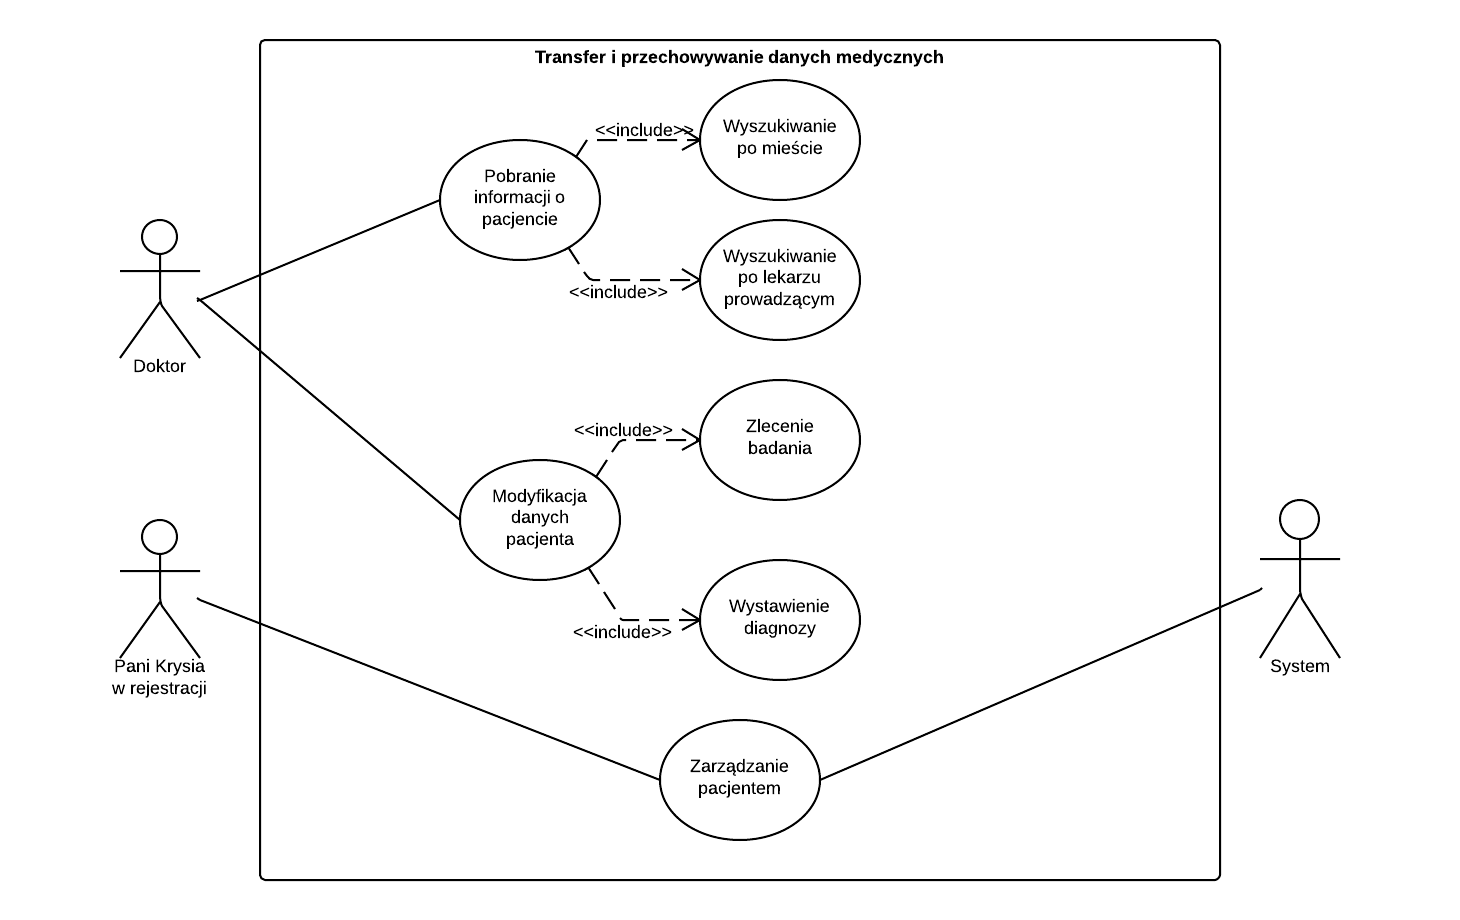
\includegraphics[width=\textwidth]{pics/UseCase}
	\caption{Diagram przypadków użycia}
	\label{fig:usecase}
\end{figure}
\begin{multicols}{2}

\subsection{Pobranie informacji o pacjencie}
\label{cha:patientinfo-usecase}

[opis]

[schemat - OWL]

[zapytanie sparql]

[metoda z klienta JAVA]